\documentclass[11pt]{standalone}
\usepackage{amssymb}
\usepackage{amsmath}
\usepackage[no-math]{fontspec}
\usepackage{unicode-math}
\setmainfont{Libertinus Sans}
\setsansfont{Libertinus Sans}
\setmathfont{Libertinus Math}
\usepackage{pgf,xcolor}
\usepackage{tikz}
\usetikzlibrary{arrows.meta, backgrounds}
\usepackage{pgfplots}
\pgfplotsset{compat=newest}
\usepackage{pifont}

\definecolor{my_darkgray}{HTML}{484949}
\definecolor{my_lightgray}{HTML}{F3F4F4}
\definecolor{my_darkblue}{HTML}{005A94}
\definecolor{my_lightblue}{HTML}{CCDEE9}
\definecolor{my_yellow}{HTML}{FFEC7F}
\definecolor{my_red}{HTML}{E60000}
\definecolor{my_orange}{HTML}{E87846}

% ---------------------------------------------------------------
% Bremsmodell: v(t) = v0 * exp(-k*t),  v0 = 100/3.6 s 27.78 m/s,  k = 0.35 1/s
% Drei Messpunkte: t = 0, 1, 2 s
%   P0 = (0,    27.7778)
%   P1 = (1,    19.5747)
%   P2 = (2,    13.7940)
%
% Parabel p(t) = 1.2112*t^2 - 9.4143*t + 27.7778
% (eindeutige Parabel durch P0, P1, P2)
%
% Skalierung der Zeichnung:
%   x-Richtung: 1 s  = 2.5 cm   =>  t in [0,2] entspricht [0,5] cm
%   y-Richtung: 1 m/s = 0.15 cm =>  v in [0,30] entspricht [0,4.5] cm
%   Hilfsmakros:
%     \tx{#1}  skaliert Zeit-Wert auf cm-Koordinate
%     \tv{#1}  skaliert Geschwindigkeits-Wert auf cm-Koordinate
% ---------------------------------------------------------------

\newcommand{\tx}[1]{(#1*2.5)}   % t -> x in cm
\newcommand{\tv}[1]{(#1*0.15)}  % v -> y in cm

\begin{document}

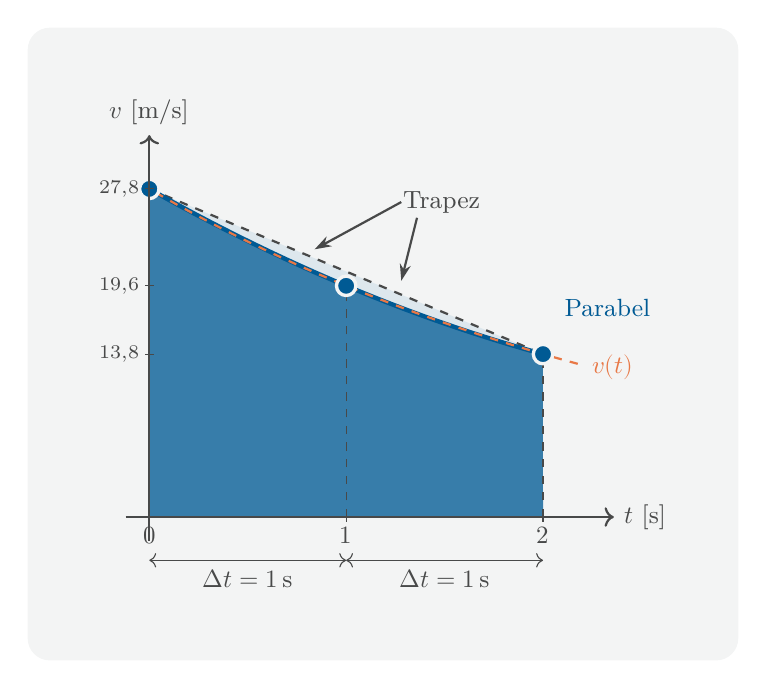
\begin{tikzpicture}[
    show background rectangle,
    background rectangle/.style={fill=my_lightgray, rounded corners=8pt},
    inner frame sep=0.8cm,
    annotation/.style={draw=my_darkgray, thick, -{Stealth[length=6pt, width=4pt]}},
]

% ==============================================================
% Koordinaten der drei Messpunkte (in Zeicheneinheiten)
% x = t * 2.5,  y = v * 0.15
% ==============================================================
\coordinate (P0) at (0.0000, 4.1667);   % t=0, v=27.7778
\coordinate (P1) at (2.5000, 2.9362);   % t=1, v=19.5747
\coordinate (P2) at (5.0000, 2.0691);   % t=2, v=13.7940

% ==============================================================
% Flaeche Trapezregel (hellblau)
% Trapez unter der Geraden P0--P2 bis zur t-Achse
% ==============================================================
\fill[my_lightblue, opacity=0.55]
    (0, 0) -- (P0) -- (P2) -- (5.0, 0) -- cycle;

% ==============================================================
% Flaeche Simpson-Regel (gelb)
% Unter der Parabel p(t) = 1.2112*t^2 - 9.4143*t + 27.7778
% x = t*2.5,  y = p(t)*0.15
% In t-Koordinaten: plot von t=0 bis t=2, dann Skala anwenden
% Ausdruck in Zeichenkoordinaten x (cm):
%   t = x/2.5
%   y = 0.15 * (1.2112*(x/2.5)^2 - 9.4143*(x/2.5) + 27.7778)
%     = 0.15 * (1.2112*x^2/6.25 - 9.4143*x/2.5 + 27.7778)
%     = 0.15 * (0.19379*x^2 - 3.76572*x + 27.7778)
%     = 0.029069*x^2 - 0.564858*x + 4.16667
% ==============================================================
\fill[my_darkblue, opacity=0.75]
    (0, 0)
    -- plot[domain=0:5, samples=80]
         (\x, {0.029069*\x*\x - 0.564858*\x + 4.16667})
    -- (5.0, 0) -- cycle;

% ==============================================================
% Trapezlinie P0--P2 (dunkelgrau, gestrichelt)
% ==============================================================
\draw[my_darkgray, dashed, thick] (P0) -- (P2);

% ==============================================================
% Parabelkurve (dunkelblau, ausgezogen)
% ==============================================================
\draw[my_darkblue, ultra thick]
    plot[domain=0:5, samples=80]
        (\x, {0.029069*\x*\x - 0.564858*\x + 4.16667});

% ==============================================================
% Echte Exponentialfunktion v(t) = 27.7778 * exp(-0.35*t)
% In Zeichenkoordinaten: t = x/2.5
%   y = 0.15 * 27.7778 * exp(-0.35 * x/2.5)
%     = 4.16667 * exp(-0.14*x)
% ==============================================================
\draw[my_orange, thick, dashed]
    plot[domain=-0.1:5.5, samples=100]
        (\x, {4.16667 * exp(-0.14*\x)});

% ==============================================================
% Senkrechte Hilfslinien zu den Messpunkten
% ==============================================================
\draw[my_darkgray, thin, dashed] (2.5, 0) -- (P1);
\draw[my_darkgray, thin, dashed] (5.0, 0) -- (P2);

% ==============================================================
% Messpunkte als Kreise
% ==============================================================
\filldraw[fill=my_darkblue, draw=my_lightgray, line width=1.2pt]
    (P0) circle (3.5pt);
\filldraw[fill=my_darkblue, draw=my_lightgray, line width=1.2pt]
    (P1) circle (3.5pt);
\filldraw[fill=my_darkblue, draw=my_lightgray, line width=1.2pt]
    (P2) circle (3.5pt);

% ==============================================================
% Achsen
% ==============================================================
\draw[->, thick, color=my_darkgray]
    (-0.3, 0) -- (5.9, 0)
    node[right, font=\small, color=my_darkgray] {$t$ [s]};
\draw[->, thick, color=my_darkgray]
    (0, -0.3) -- (0, 4.85)
    node[above, font=\small, color=my_darkgray] {$v$ [m/s]};

% ==============================================================
% Achsenbeschriftungen
% ==============================================================
% t-Achse: Zeitwerte
\foreach \tval/\xval in {1/2.5, 2/5.0} {
    \draw[my_darkgray, thin] (\xval, 0.06) -- (\xval, -0.06);
    \node[below, font=\small, color=my_darkgray] at (\xval, 0) {$\tval$};
}
\node[below, font=\small, color=my_darkgray] at (0, 0) {$0$};

% v-Achse: Geschwindigkeitswerte an den drei Messpunkten
\draw[my_darkgray, thin] (0.06, 4.1667) -- (-0.06, 4.1667);
\node[left, font=\scriptsize, color=my_darkgray] at (0, 4.1667)
    {$27{,}8$};

\draw[my_darkgray, thin] (0.06, 2.9362) -- (-0.06, 2.9362);
\node[left, font=\scriptsize, color=my_darkgray] at (0, 2.9362)
    {$19{,}6$};

\draw[my_darkgray, thin] (0.06, 2.0691) -- (-0.06, 2.0691);
\node[left, font=\scriptsize, color=my_darkgray] at (0, 2.0691)
    {$13{,}8$};

% ==============================================================
% Annotationen
% ==============================================================

% Echte Kurve v(t)
\node[font=\small, color=my_orange, anchor=west]
    at (5.5, 1.9) {$v(t)$};

% Parabel
\node[font=\small, color=my_darkblue, anchor=west]
    at (5.15, 2.65) {Parabel};

% Trapez-Label mit Pfeil auf die Trapezflaeche
\node[font=\small, color=my_darkgray, anchor=west]
    at (3.1, 4.0) {Trapez};
\draw[annotation] (3.2, 4.0) -- (2.1, 3.4);
\draw[annotation] (3.4, 3.8) -- (3.2, 3.0);

% Flaechen-Labels
%\node[font=\footnotesize, color=my_darkgray, anchor=center]
%    at (1.2, 0.4) {Trapezfläche};
%\node[font=\footnotesize, color=my_darkgray, anchor=center]
%    at (2.5, 1.15) {Simpsonfläche};

% Delta t Bemaßung
\draw[<->, my_darkgray, thin]
    (0, -0.55) -- (2.5, -0.55)
    node[midway, below, font=\small, color=my_darkgray] {$\Delta t = 1\,\text{s}$};
\draw[<->, my_darkgray, thin]
    (2.5, -0.55) -- (5.0, -0.55)
    node[midway, below, font=\small, color=my_darkgray] {$\Delta t = 1\,\text{s}$};

% Mittelpunkt-Gewicht Annotation
%\node[font=\footnotesize\bfseries, color=my_darkblue, above right]
%    at (P1) {$\times 4$};

\end{tikzpicture}
\end{document}
